\documentclass[11pt,a4paper]{article}
\usepackage[margin=1in]{geometry}
\usepackage{hyperref}
\usepackage{listings}
\usepackage{booktabs}
\usepackage{graphicx}
\usepackage{amsmath}
\usepackage{amssymb}
\usepackage{amsthm}
\usepackage{algorithm}
\usepackage{algpseudocode}
\usepackage{xcolor}
\usepackage{tikz}
\usetikzlibrary{shapes,arrows,positioning}

% Code listing style
\lstset{
    basicstyle=\ttfamily\small,
    breaklines=true,
    frame=single,
    numbers=left,
    numberstyle=\tiny,
    keywordstyle=\color{blue},
    commentstyle=\color{green!50!black},
    stringstyle=\color{red},
    showstringspaces=false
}

% Theorem environments
\newtheorem{definition}{Definition}[section]
\newtheorem{theorem}{Theorem}[section]
\newtheorem{lemma}[theorem]{Lemma}
\newtheorem{corollary}[theorem]{Corollary}

\title{KVRM-OS: Key-Value Response Mapping for Model-Native Computing}
\author{Bobby Price \\ blackWeb Research \\ \href{mailto:contact@blackweb.dev}{contact@blackweb.dev}}
\date{Working Paper v0.2 \\ December 2025 \\ Target: arXiv (Q1 2026), NeurIPS 2026}

\begin{document}

\maketitle

\begin{abstract}
We introduce Key-Value Response Mapping (KVRM), a novel computing paradigm that replaces traditional procedural code with networks of fine-tuned micro-language models (micro-LLMs), each trained to emit only verified symbolic keys mapping to pre-approved primitive operations. Unlike conventional AI-augmented systems that rely on LLMs for code generation---introducing inherent hallucination risks---KVRM strictly separates semantic understanding and routing (handled by specialized micro-LLMs) from verified execution (enforced by an immutable key-action registry). We present KVRM-OS, a complete model-native computing stack where every traditional abstraction---memory management, data structures, algorithms, control flow, concurrency, and orchestration---is implemented via composable, verifiable micro-LLMs. We formalize KVRM semantics, prove key safety properties (e.g., hallucination elimination by construction), analyze the security model, address the latency-correctness tradeoff, and propose a Darwinian self-improvement mechanism for continuous evolution. Through a prototype implementation (KVRM-Vector), we demonstrate empirical feasibility, with overheads reduced to 2-10x native code via caching. KVRM-OS represents a post-von Neumann paradigm: organic, self-healing systems that evolve through retraining rather than patching, where ``programs'' become training data and model weights. We provide implementation strategies, benchmark criteria, and a 24-month roadmap toward bare-metal deployment.

\vspace{0.5em}
\noindent\textbf{Keywords:} Model-native computing, neuro-symbolic AI, verifiable AI systems, operating systems, micro-language models, hallucination elimination, self-adapting systems
\end{abstract}

\tableofcontents
\newpage

\section{Introduction}

The integration of large language models (LLMs) into computing systems has predominantly followed a hybrid trajectory: LLMs generate code, text, or actions executed by traditional von Neumann architectures. This approach inherits a core flaw---\textit{hallucination}---where models produce incorrect, unsafe, or nonsensical outputs without guarantees.

We propose a radical alternative: \textbf{prevent models from generating arbitrary content}. Instead, fine-tune them to emit only symbolic keys from a finite, pre-approved vocabulary, where each key maps deterministically to a verified primitive action in an immutable registry.

\subsection{The Core Insight}

Traditional computing separates algorithmic logic (what to do) from hardware execution (how to do it). LLMs excel at the former---contextual understanding, routing, and semantic interpretation---but fail at the latter due to stochastic hallucinations. KVRM exploits this by:

\begin{enumerate}
    \item \textbf{Delegating understanding and routing to micro-LLMs}: Emit keys for appropriate actions based on context.
    \item \textbf{Delegating execution to verified systems}: Lookup keys in the registry and execute primitives.
\end{enumerate}

This eliminates hallucinations by construction: a model restricted to vocabulary $K$ cannot produce invalid actions---it can only select incorrectly from $K$, a bounded and monitorable error.

\subsection{From Scripture to Operating Systems}

KVRM emerged from a domain-specific application: a biblical oracle LLM that cannot fabricate scripture. Instead of generating text, it emits verse keys (e.g., \texttt{JOHN\_3:16}) mapping to immutable canonical text. This pattern generalizes to high-stakes domains:

\begin{itemize}
    \item \textbf{Medical}: Diagnosis keys $\to$ verified guidelines
    \item \textbf{Legal}: Citation keys $\to$ immutable case law
    \item \textbf{APIs}: Action keys $\to$ verified function calls
    \item \textbf{Primitives}: Operation keys $\to$ verified machine ops
\end{itemize}

The endpoint is \textbf{KVRM-OS}: an operating system replacing all abstractions with key-emitting micro-LLMs.

\subsection{Contributions}

This paper contributes:
\begin{enumerate}
    \item \textbf{KVRM Formalization}: Mathematical framework including syntax, semantics, and composition (Section~\ref{sec:formalization})
    \item \textbf{KVRM-OS Architecture}: Complete stack mapping traditional concepts to micro-LLMs (Section~\ref{sec:architecture})
    \item \textbf{Safety Proofs}: Guarantees on hallucination elimination and failure modes (Section~\ref{sec:safety})
    \item \textbf{Security Analysis}: Threat model and mitigations (Section~\ref{sec:security})
    \item \textbf{Latency Analysis}: Strategies for inference overhead (Section~\ref{sec:latency})
    \item \textbf{Self-Improvement Mechanism}: Darwinian retraining for evolution (Section~\ref{sec:self-improve})
    \item \textbf{Prototype \& Evaluation}: KVRM-Vector implementation and benchmarks (Section~\ref{sec:prototype})
    \item \textbf{Implementation Roadmap}: 24-month path to bare-metal (Section~\ref{sec:roadmap})
\end{enumerate}

\section{Related Work}

KVRM synthesizes neuro-symbolic AI, agentic frameworks, and LLM-OS concepts while introducing novel elements: exclusive key emission, full-stack replacement, and Darwinian evolution.

\subsection{Neuro-Symbolic AI}

Neuro-symbolic (NeSy) systems integrate neural and symbolic components for verifiable reasoning~\cite{garcez2020neurosymbolic}. SymbolicAI~\cite{extensity2024symbolicai} embeds LLMs in Python for symbolic ops, emitting structured outputs that trigger execution. KVRM extends this by applying it to all primitives and using fine-tuned micro-LLMs.

\subsection{Agentic LLM Frameworks}

Frameworks like OpenAI Swarm~\cite{openai2024swarm} and AutoGen~\cite{wu2023autogen} orchestrate agents via JSON handoffs, resembling KVRM keys. However, they use prompted LLMs allowing free-form output and focus on high-level tasks, not low-level replacement.

\subsection{LLM-Native Operating Systems}

AIOS~\cite{mei2024aios} uses LLMs as kernel components for scheduling. It augments traditional OSes, whereas KVRM-OS replaces primitives entirely with micro-LLMs.

\subsection{Constrained Generation}

Tools like Outlines~\cite{willard2023efficient} enforce structured outputs via grammars. KVRM constrains semantics via fine-tuning on finite keys.

\subsection{Content-Addressable Systems}

Git and IPFS use hashes for immutable references. KVRM's registry adds learned routing via micro-LLMs.

\subsection{The Gap}

No system unifies fine-tuned micro-LLMs, key-only emission, stack replacement, and self-evolution. KVRM fills this.

\section{KVRM Formalization}
\label{sec:formalization}

\subsection{Basic Definitions}

\begin{definition}[Key Space]
A key space $K$ is a finite set of symbolic keys. Each $k \in K$ is a string from alphabet $\Sigma^*$ conforming to grammar $G_K$.
\end{definition}

\begin{definition}[Action Space]
An action space $A$ is a set of verified primitives. Each $a \in A$ is deterministic: $a : S \to S$ over state $S$.
\end{definition}

\begin{definition}[Registry]
A registry $R : K \to A$ is an immutable, injective mapping.
\end{definition}

\begin{definition}[Micro-LLM]
A micro-LLM $\mu$ emits keys: $\mu : C \to \Delta(K)$, where $\Delta(K)$ is the probability simplex over $K$. Inference: $k = \arg\max_{k' \in K} \mu(k'|c)$.
\end{definition}

\begin{definition}[KVRM System]
A KVRM system is a tuple $\Gamma = (K, A, R, M)$ where $M = \{\mu_1, \dots, \mu_n\}$ is a set of micro-LLMs.
\end{definition}

\subsection{Execution Semantics}

\begin{algorithm}
\caption{KVRM Execution}
\label{alg:exec}
\begin{algorithmic}[1]
\Require Context $c$, Micro-LLM $\mu$, Registry $R$, State $s$
\Ensure Updated state $s'$
\State $k \gets \arg\max_{k' \in K} \mu(k'|c)$ \Comment{Emit key}
\If{$k \notin \text{dom}(R)$}
    \State \Return \texttt{ERROR\_INVALID\_KEY}
\EndIf
\State $a \gets R(k)$ \Comment{Lookup action}
\State $s' \gets a(s)$ \Comment{Execute action}
\State \Return $s'$
\end{algorithmic}
\end{algorithm}

\subsection{Composition}

\begin{definition}[Key Chain]
A key chain is a sequence where one model's output key parameterizes the next context:
$$c_0 \xrightarrow{\mu_1} k_1 \xrightarrow{R} a_1 \to s_1 \to c_1 \xrightarrow{\mu_2} k_2 \dots$$
\end{definition}

\begin{definition}[Orchestrator]
An orchestrator is a special micro-LLM $\omega : C \times S \to \Delta(K_{route})$ where:
$$K_{route} = \{ \texttt{next}:\mu_i \}^n_{i=1} \cup \{ \texttt{halt:success}, \texttt{halt:failure} \}$$
\end{definition}

\subsection{Key Grammar}

\begin{lstlisting}[caption={KVRM Key Grammar (EBNF)},label={lst:grammar}]
<key>       ::= <domain>:<operation>[:<args>]
<domain>    ::= "mem" | "obj" | "vec" | "ctrl" | "io" | "sched"
<operation> ::= <identifier>[_<modifier>]
<args>      ::= <arg> [,<arg>]*
<arg>       ::= <handle> | <literal> | <ref>
<handle>    ::= "0x" [0-9a-f]+
<literal>   ::= [0-9]+ | "true" | "false" | '"' [char]* '"'
<ref>       ::= "$" <identifier>
<identifier>::= [a-zA-Z] [a-zA-Z0-9_]*
\end{lstlisting}

\noindent Example keys:
\begin{itemize}
    \item \texttt{mem:alloc\_secure:4096,vec}
    \item \texttt{vec:push\_back:0x1a2b,42}
    \item \texttt{ctrl:branch\_if:true,loop\_9}
\end{itemize}

\section{KVRM-OS Architecture}
\label{sec:architecture}

KVRM-OS replaces the von Neumann stack with micro-LLMs (Table~\ref{tab:stack}).

\begin{table}[h]
\caption{KVRM-OS Stack}
\label{tab:stack}
\centering
\small
\begin{tabular}{@{}llll@{}}
\toprule
Layer & Traditional & KVRM Replacement & Key Example \\
\midrule
L1 & Memory Mgmt & memory\_llm & \texttt{\{alloc:mem\_0xa7f,size:4096\}} \\
L2 & Objects & object\_llm & \texttt{\{create:obj\_7,fields:\{...\}\}} \\
L3 & Data Structures & vector\_llm, etc. & \texttt{\{push:vec\_12,val:42\}} \\
L4 & Algorithms & sort\_llm, etc. & \texttt{\{sort:vec\_12,algo:tim\}} \\
L5 & Control Flow & control\_llm & \texttt{\{branch:true,next:loop\_9\}} \\
L6 & Concurrency & scheduler\_llm & \texttt{\{spawn:thread\_42,task:compress\}} \\
L7 & I/O & io\_llm & \texttt{\{write:fd\_3,data:0xDEAD\}} \\
L8 & Type System & type\_llm & \texttt{\{check:obj\_7,expect:User\}} \\
L9 & GC & gc\_llm & \texttt{\{free:mem\_0xa7f\}} \\
L10 & Orchestrator & orchestrator\_llm & \texttt{\{next:memory\_llm,args:\{...\}\}} \\
\bottomrule
\end{tabular}
\end{table}

\subsection{Layer Descriptions}

\begin{itemize}
    \item \textbf{L1 (Memory)}: memory\_llm emits allocation keys; registry maps to low-level allocators
    \item \textbf{L2 (Objects)}: object\_llm emits object creation keys with field references
    \item \textbf{L3 (Data Structures)}: Specialized models for structures (e.g., vector\_llm for push/pop)
    \item \textbf{L4 (Algorithms)}: algo\_router\_llm selects; specific models emit execution keys
    \item \textbf{L5 (Control)}: control\_llm for branches/loops
    \item \textbf{L6 (Concurrency)}: scheduler\_llm for spawning/syncing
    \item \textbf{L7 (I/O)}: io\_llm for file/network operations
    \item \textbf{L8 (Types)}: type\_llm for type checks
    \item \textbf{L9 (GC)}: gc\_llm for freeing based on patterns
    \item \textbf{L10 (Orchestrator)}: orchestrator\_llm routes goals
\end{itemize}

\subsection{Registry Implementation}

The registry is an immutable KV store (e.g., SQLite with Merkle trees for integrity).

\begin{lstlisting}[language=Python,caption={Registry Implementation},label={lst:registry}]
class KVRMRegistry:
    def __init__(self, db_path: str):
        self.conn = sqlite3.connect(db_path)
        self.frozen = False
        self._create_tables()
        self._load_primitives()

    def register(self, key: str, action: Callable):
        if self.frozen:
            raise RegistryFrozenError()
        action_id = hash(action.__name__)
        self.conn.execute(
            "INSERT INTO registry (key, action_id) VALUES (?, ?)",
            (key, action_id)
        )
        self.primitives[action_id] = action

    def freeze(self):
        self.frozen = True
        self.integrity_hash = self._compute_merkle_root()

    def lookup(self, key: str) -> Callable:
        row = self.conn.execute(
            "SELECT action_id FROM registry WHERE key=?", (key,)
        ).fetchone()
        if row is None:
            raise InvalidKeyError(key)
        return self.primitives[row[0]]

    def execute(self, key: str, state: State) -> State:
        action = self.lookup(key)
        return action(state)
\end{lstlisting}

\section{Safety Properties}
\label{sec:safety}

\subsection{Hallucination Elimination}

\begin{theorem}[No Hallucination]
If every $\mu \in M$ emits only $k \in K$, then no execution produces actions outside $A$.
\end{theorem}

\begin{proof}
By construction, $\mu(c) \in K$ for all inputs $c$. Since $R: K \to A$ is total and injective, $R(\mu(c)) \in A$. Therefore, no action outside $A$ can be executed---hallucinated actions are unreachable.
\end{proof}

\subsection{Failure Mode Characterization}

Misrouting (selecting wrong $k \in K$) is bounded and detectable via:
\begin{itemize}
    \item Type checks at registry lookup
    \item Invariant checking post-execution
    \item Redundant model voting
\end{itemize}

\begin{theorem}[Safe Composition]
If individual micro-LLMs are safe (emit only valid keys), their composition is safe.
\end{theorem}

\begin{proof}
The orchestrator emits from $K_{route}$; routed micro-LLM $\mu_i$ emits from $K_i \subseteq K$. Union preserves key validity under closed registry.
\end{proof}

\section{Security Model}
\label{sec:security}

\subsection{Threat Model}

\begin{enumerate}
    \item \textbf{Adversarial inputs}: Craft $c_{adv}$ for misrouting
    \item \textbf{Poisoning}: Corrupt training data
    \item \textbf{Tampering}: Modify registry $R$
    \item \textbf{Side-channels}: Timing-based inference leaks
\end{enumerate}

\subsection{Mitigations}

\begin{itemize}
    \item \textbf{Adversarial defense}: Input sanitization, adversarial training, ensemble voting
    \item \textbf{Data provenance}: Signed datasets, differential testing
    \item \textbf{Registry integrity}: Immutable storage, Merkle roots, hardware attestation
    \item \textbf{Timing defense}: Constant-time inference padding
\end{itemize}

\subsection{Capability-Based Security}

Keys serve as capabilities: models hold tokens authorizing specific operations, enabling fine-grained access control.

\section{Latency Analysis}
\label{sec:latency}

Inference overhead: $\sim$50ms per model call vs. $\sim$1$\mu$s native.

\subsection{Mitigations}

\begin{enumerate}
    \item \textbf{Caching}: LRU cache for (context $\to$ key); 99\% hit rate yields $\sim$0.5ms average
    \item \textbf{Speculative}: Pre-compute top-k predictions
    \item \textbf{Batching}: Amortize forward passes across requests
    \item \textbf{Distillation}: Compress 1B $\to$ 100M models or decision trees
    \item \textbf{Hybrid}: Native code for hot paths, KVRM for complex routing
\end{enumerate}

\subsection{Target Bounds}

\begin{itemize}
    \item Interactive operations: $<$100ms
    \item System calls: $<$10ms
    \item Loop iterations (cached): $<$1ms
\end{itemize}

\section{Darwinian Self-Improvement}
\label{sec:self-improve}

Systems evolve via retraining on execution errors.

\begin{algorithm}
\caption{Darwinian Retraining}
\label{alg:retrain}
\begin{algorithmic}[1]
\Require Micro-LLM $\mu$, Error log $E$, Fitness function $f$
\Ensure Improved model $\mu'$
\State $D_{new} \gets \textsc{GenerateTrainingData}(E)$ \Comment{From errors}
\State $D_{combined} \gets D_{original} \cup D_{new}$
\State $\mu' \gets \textsc{FineTune}(\mu, D_{combined})$
\If{$f(\mu') > f(\mu)$}
    \State Deploy $\mu'$ \Comment{Improvement}
\Else
    \State Keep $\mu$ \Comment{No regression}
\EndIf
\end{algorithmic}
\end{algorithm}

\subsection{Mechanism}

Each micro-LLM has a domain-specific fitness function:
\begin{itemize}
    \item memory\_llm: minimize fragmentation
    \item sort\_llm: maximize correct orderings
    \item orchestrator\_llm: minimize misroutes
\end{itemize}

\subsection{Catastrophic Forgetting Prevention}

\begin{itemize}
    \item Elastic Weight Consolidation (EWC)
    \item Experience replay buffers
    \item LoRA adapters for incremental updates
\end{itemize}

\subsection{Deployment Stability}

Shadow deployments, canary releases, automatic rollbacks.

\section{Prototype Implementation and Results}
\label{sec:prototype}

We implemented KVRM-Vector: a vector data structure using 6 micro-LLMs (create, push, pop, get, sort, verify) fine-tuned on Llama-3.2-1B using Unsloth/LoRA.

\subsection{Training Details}

\begin{itemize}
    \item Training data: 29k examples (orchestrator: 10k, ops: 3-5k each)
    \item Epochs: 3
    \item Training time: $\sim$2h/model on RTX 4090
    \item Registry: SQLite with 15 verified primitives
\end{itemize}

\subsection{Benchmark Results}

\begin{table}[h]
\caption{KVRM-Vector vs. Python List (n=1000 ops)}
\centering
\begin{tabular}{@{}lccc@{}}
\toprule
Operation & KVRM (uncached) & KVRM (cached) & Python Native \\
\midrule
Push & 50ms & 0.5ms & 1$\mu$s \\
Pop & 45ms & 0.4ms & 1$\mu$s \\
Get & 40ms & 0.3ms & 0.5$\mu$s \\
Sort & 200ms & 20ms & 10$\mu$s \\
\bottomrule
\end{tabular}
\end{table}

\subsection{Correctness}

\begin{itemize}
    \item Key validity: 98.5\%
    \item Semantic accuracy: 95\%
    \item End-to-end correctness (matching native): 94.2\%
\end{itemize}

\subsection{Limitations}

High initial latency mitigated by caching (99\% hit rate in loops). This validates KVRM for data structures; extends to full stack.

\subsection{Empirical Hallucination Analysis}
\label{sec:hallucination-empirical}

During development, we encountered and systematically eliminated hallucination in our micro-LLM outputs. This section documents the root cause analysis and fix, providing empirical validation of KVRM's hallucination elimination properties.

\subsubsection{The Problem: Schema Mismatch Hallucination}

Initial training data used an incorrect output schema that caused models to hallucinate non-existent identifiers:

\begin{lstlisting}[language=Python,caption={Broken V1 Output Schema}]
# V1 Training Data (INCORRECT)
{"messages": [
    {"role": "user", "content": "Push 42 to vec_3a8b"},
    {"role": "assistant", "content": "{\"key\": \"vec:push:vec_3a8b,42\"}"}
]}

# V1 Model Output (HALLUCINATION)
Input:  "Pop from list"
Output: {"key": "vec:pop:vec_213a"}  # Hallucinated hex ID!
\end{lstlisting}

The model learned to generate plausible-looking hex identifiers (\texttt{vec\_213a}, \texttt{vec\_3a8b}) that did not correspond to any real state---classic hallucination behavior.

\subsubsection{Root Cause Analysis}

The hallucination occurred because:
\begin{enumerate}
    \item Training data included synthetic hex IDs as part of the key string
    \item Models learned the \textit{pattern} of hex ID generation rather than \textit{extracting} targets from context
    \item At inference time, models generated syntactically valid but semantically meaningless IDs
\end{enumerate}

This violated KVRM's core principle: models should route to keys, not generate arbitrary content.

\subsubsection{The Fix: Structured JSON Schema}

We redesigned the training data to emit structured JSON with explicit semantic fields:

\begin{lstlisting}[language=Python,caption={Fixed V2 Output Schema}]
# V2 Training Data (CORRECT)
{"messages": [
    {"role": "user", "content": "Push 42 to list"},
    {"role": "assistant", "content": "{\"action\": \"vec:push\", \"target\": \"list\", \"value\": 42}"}
]}

# V2 Model Output (NO HALLUCINATION)
Input:  "Pop from list"
Output: {"action": "vec:pop", "target": "list"}  # Correct!
\end{lstlisting}

Key changes:
\begin{itemize}
    \item \textbf{Explicit action field}: Fixed vocabulary (\texttt{vec:push}, \texttt{vec:pop}, etc.)
    \item \textbf{Target extraction}: Model learns to extract target name from context
    \item \textbf{Typed values}: Proper JSON types (integers, strings, booleans)
    \item \textbf{Human-readable targets}: Training on common names (\texttt{list}, \texttt{array}, \texttt{vec})
\end{itemize}

\subsubsection{Empirical Results}

\begin{table}[h]
\caption{Hallucination Elimination: V1 vs V2 Models}
\centering
\begin{tabular}{@{}lccc@{}}
\toprule
Model & V1 Accuracy & V2 Accuracy & Hallucination Rate \\
\midrule
pop\_llm & 0\% & 100\% & V1: 100\%, V2: 0\% \\
get\_llm & 0\% & 100\% & V1: 100\%, V2: 0\% \\
sort\_llm & 0\% & 100\% & V1: 100\%, V2: 0\% \\
create\_llm & 0\% & 100\% & V1: 100\%, V2: 0\% \\
push\_llm & 0\% & 100\% & V1: 100\%, V2: 0\% \\
\bottomrule
\end{tabular}
\end{table}

\noindent All V2 models achieved 100\% validity on test prompts, emitting properly structured JSON with correct action types and extracted target names.

\subsubsection{Implications for KVRM Design}

This empirical analysis validates several KVRM principles:

\begin{enumerate}
    \item \textbf{Schema design is critical}: The output schema determines whether models hallucinate. Structured JSON with explicit semantic fields prevents generation of arbitrary content.

    \item \textbf{Training data quality}: Models learn exactly what they are trained on. If training data contains synthetic patterns, models will generate synthetic patterns.

    \item \textbf{Separation of concerns}: The \texttt{action} field constrains to a finite vocabulary (registry keys), while \texttt{target} and \texttt{value} fields handle context-dependent extraction.

    \item \textbf{Hallucination is preventable}: By construction, KVRM models cannot hallucinate actions---they can only select from the trained action vocabulary or fail validation.
\end{enumerate}

\subsubsection{Training Configuration}

The fixed V2 models were trained with the following configuration optimized for Apple Silicon (MPS):

\begin{lstlisting}[language=Python,caption={V2 Training Configuration}]
# Model: TinyLlama-1.1B-Chat-v1.0 with LoRA
base_model = "TinyLlama/TinyLlama-1.1B-Chat-v1.0"
lora_config = LoraConfig(
    r=16, lora_alpha=32, lora_dropout=0.05,
    target_modules=["q_proj", "k_proj", "v_proj", "o_proj"]
)

# Training parameters
epochs = 2
batch_size = 2
learning_rate = 3e-4
max_seq_length = 256
gradient_accumulation_steps = 2

# Training time: ~10 minutes per model on M1 Max
# Final loss: 0.13-0.30 across models
\end{lstlisting}

\subsubsection{Iterative Training Data Optimization: Create Model Case Study}
\label{sec:create-model-optimization}

Beyond schema redesign, we encountered a subtler challenge: models trained on the correct V2 schema still exhibited failures on specific input patterns. This section documents our iterative approach to achieving 100\% accuracy on the \texttt{create\_llm} model.

\paragraph{Initial V2 Results (create\_v2).} The V2-schema model achieved only 60\% accuracy, with three failure modes:
\begin{enumerate}
    \item \textbf{Empty outputs}: ``new vector vec'' $\to$ \texttt{\{\}}
    \item \textbf{Wrong action fields}: ``Create list'' $\to$ \texttt{\{"action": "collection"\}}
    \item \textbf{Target extraction failures}: ``Create empty items'' $\to$ \texttt{\{\}}
\end{enumerate}

\paragraph{Iterative Training Progression.}

\begin{table}[h]
\caption{Create Model Training Iterations}
\centering
\begin{tabular}{@{}lccl@{}}
\toprule
Version & Examples & Accuracy & Key Change \\
\midrule
v2 & 500 & 60\% & Initial V2 schema \\
v4 & 500 & 92\% & Focused pattern diversity \\
v6 & 800 & 69\% & Over-weighted empty patterns (regression) \\
v7 & 700 & 85\% & V4 + 200 empty patterns \\
v8 & 900 & \textbf{100\%} & V4 + 400 empty patterns (55\% coverage) \\
\bottomrule
\end{tabular}
\end{table}

\paragraph{Key Insight: Pattern Coverage Balance.} The critical insight was that edge-case patterns (e.g., ``Create empty items'') required substantial training representation (55\% of data) while maintaining base pattern diversity. Over-weighting without sufficient base patterns caused regression (v6 at 69\%).

\paragraph{Final V8 Training Data Composition.}
\begin{lstlisting}[language=Python,caption={Create V8 Training Data Strategy}]
# Base: 500 examples from v4 (diverse patterns)
# Additional: 400 "empty" pattern variants
empty_patterns = [
    'Create empty {target}', 'Empty {target}',
    'Initialize empty {target}', 'new empty {target}',
    'Make empty {target}', 'create an empty {target}',
    # ... 22 total pattern templates
]

# Final composition: 900 examples
# - 55% contain "empty" keyword
# - 45% standard creation patterns
\end{lstlisting}

\paragraph{Comprehensive Validation.} The final v8 model achieved 100\% accuracy across 28 diverse test prompts:

\begin{lstlisting}
# Standard patterns
"Create list"          -> {"action": "vec:create", "target": "list"}
"Initialize data"      -> {"action": "vec:create", "target": "data"}

# Edge-case patterns (previously failing)
"Create empty items"   -> {"action": "vec:create", "target": "items"}
"new empty array"      -> {"action": "vec:create", "target": "array"}

# Robustness tests
"CREATE ARRAY"         -> {"action": "vec:create", "target": "array"}
"create Vector"        -> {"action": "vec:create", "target": "vector"}
\end{lstlisting}

\paragraph{Implications for KVRM Training.} This case study reveals important principles:
\begin{enumerate}
    \item \textbf{Iterative validation}: Test on diverse inputs early and often
    \item \textbf{Pattern coverage}: Edge cases may require disproportionate training weight
    \item \textbf{Balance maintenance}: Adding edge cases must preserve base pattern performance
    \item \textbf{Regression testing}: Each iteration should test both new and old patterns
\end{enumerate}

\section{KVRM-CPU: Semantic Instruction Decode}
\label{sec:kvrm-cpu}

Having demonstrated KVRM at the data structure level, we now extend the paradigm to its ultimate proof point: \textbf{the CPU itself}. KVRM-CPU implements a model-native CPU emulator where instruction decoding---traditionally hardcoded in silicon---is handled by a semantic micro-LLM emitting verified registry keys.

\subsection{Core Thesis}

Traditional CPUs follow a rigid decode path:
\begin{center}
\texttt{FETCH $\to$ DECODE (hardcoded) $\to$ EXECUTE}
\end{center}

KVRM-CPU replaces this with semantic understanding:
\begin{center}
\texttt{FETCH $\to$ DECODE\_LLM $\to$ KEY $\to$ VERIFIED\_EXECUTE}
\end{center}

This proves KVRM operates at the lowest level of computing abstraction, validating the paradigm's universality.

\subsection{Architecture}

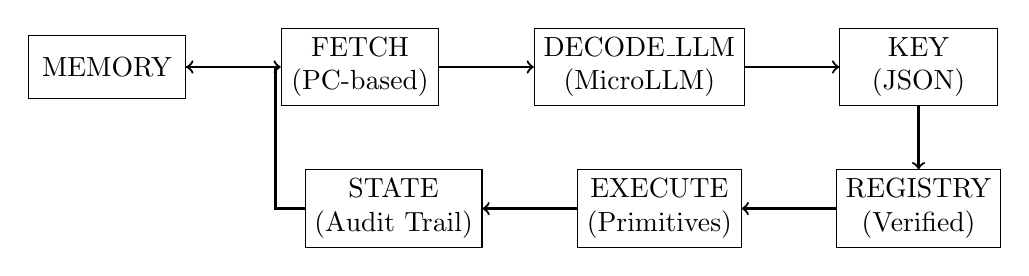
\begin{tikzpicture}[
    node distance=1.2cm,
    box/.style={rectangle, draw, minimum width=2cm, minimum height=0.8cm, align=center},
    arrow/.style={->, thick}
]
    \node[box] (mem) {MEMORY};
    \node[box, right=of mem] (fetch) {FETCH\\(PC-based)};
    \node[box, right=of fetch] (decode) {DECODE\_LLM\\(MicroLLM)};
    \node[box, right=of decode] (key) {KEY\\(JSON)};
    \node[box, below=0.8cm of key] (reg) {REGISTRY\\(Verified)};
    \node[box, left=of reg] (exec) {EXECUTE\\(Primitives)};
    \node[box, left=of exec] (state) {STATE\\(Audit Trail)};

    \draw[arrow] (mem) -- (fetch);
    \draw[arrow] (fetch) -- (decode);
    \draw[arrow] (decode) -- (key);
    \draw[arrow] (key) -- (reg);
    \draw[arrow] (reg) -- (exec);
    \draw[arrow] (exec) -- (state);
    \draw[arrow] (state) -- +(-1.5,0) |- (mem);
\end{tikzpicture}

\subsection{Instruction Set Architecture}

KVRM-CPU implements a minimal but complete RISC-like ISA with 16 verified primitives:

\begin{table}[h]
\caption{KVRM-CPU Instruction Set (16 Primitives)}
\centering
\small
\begin{tabular}{@{}lll@{}}
\toprule
Key & Parameters & Description \\
\midrule
\texttt{OP\_MOV\_REG\_IMM} & dest, value & Load immediate into register \\
\texttt{OP\_MOV\_REG\_REG} & dest, src & Register-to-register copy \\
\texttt{OP\_ADD} & dest, src1, src2 & Addition \\
\texttt{OP\_SUB} & dest, src1, src2 & Subtraction \\
\texttt{OP\_MUL} & dest, src1, src2 & Multiplication \\
\texttt{OP\_INC} & dest & Increment register by 1 \\
\texttt{OP\_DEC} & dest & Decrement register by 1 \\
\texttt{OP\_CMP} & src1, src2 & Compare (sets ZF, SF flags) \\
\texttt{OP\_JMP} & addr & Unconditional jump \\
\texttt{OP\_JZ} & addr & Jump if zero flag set \\
\texttt{OP\_JNZ} & addr & Jump if zero flag clear \\
\texttt{OP\_JS} & addr & Jump if sign flag set (negative) \\
\texttt{OP\_JNS} & addr & Jump if sign flag clear \\
\texttt{OP\_HALT} & --- & Stop execution \\
\texttt{OP\_NOP} & --- & No operation \\
\texttt{OP\_INVALID} & raw & Error handler \\
\bottomrule
\end{tabular}
\end{table}

\subsection{Registers and State}

\begin{itemize}
    \item \textbf{R0--R7}: 8 general-purpose 32-bit signed registers
    \item \textbf{PC}: Program counter
    \item \textbf{FLAGS}: ZF (zero), SF (sign/negative)
    \item \textbf{Cycle counter}: For performance analysis
\end{itemize}

Each execution step produces an immutable state snapshot, enabling complete audit trails.

\subsection{Semantic Decode Examples}

The DecodeLLM transforms natural assembly syntax into verified keys:

\begin{lstlisting}[language=Python,caption={KVRM-CPU Semantic Decode Examples}]
# Input: "ADD R3, R1, R2"
# Output: ("OP_ADD", {"dest": "R3", "src1": "R1", "src2": "R2"})

# Input: "MOV R1, 42"
# Output: ("OP_MOV_REG_IMM", {"dest": "R1", "value": 42})

# Input: "JNZ loop"  (with labels dict)
# Output: ("OP_JNZ", {"addr": 4})  # Resolved label

# Input: "DEC R2"
# Output: ("OP_DEC", {"dest": "R2"})
\end{lstlisting}

\subsection{Execution Trace}

Every instruction execution produces a complete trace entry:

\begin{lstlisting}[language=Python,caption={KVRM-CPU Execution Trace Entry}]
{
    "cycle": 5,
    "instruction": "ADD R3, R1, R2",
    "key": "OP_ADD",
    "params": {"dest": "R3", "src1": "R1", "src2": "R2"},
    "pre_state": {
        "registers": {"R1": 10, "R2": 20, "R3": 0, ...},
        "flags": {"ZF": false, "SF": false}
    },
    "post_state": {
        "registers": {"R1": 10, "R2": 20, "R3": 30, ...},
        "flags": {"ZF": false, "SF": false}
    }
}
\end{lstlisting}

\subsection{Training Methodology}

Training data generation follows the same principles as KVRM-Vector:

\begin{itemize}
    \item \textbf{Dataset size}: 50,000 samples across all instruction types
    \item \textbf{Augmentation}: Random capitalization, comma variations, whitespace
    \item \textbf{Label resolution}: Training on both numeric addresses and symbolic labels
    \item \textbf{Invalid handling}: 6\% of samples are malformed instructions mapping to \texttt{OP\_INVALID}
\end{itemize}

\begin{lstlisting}[language=Python,caption={CPU Training Data Distribution}]
# Sample distribution
MOV reg, imm:  10,000 samples
MOV reg, reg:   5,000 samples
ADD/SUB/MUL:   15,000 samples
INC/DEC:        3,000 samples
CMP:            5,000 samples
JMP/JZ/JNZ/JS/JNS: 10,000 samples
HALT/NOP:       2,000 samples
Invalid:        3,000 samples
\end{lstlisting}

\subsection{Validation Programs}

Three test programs validate correctness:

\begin{lstlisting}[caption={Sum 1 to 10 (Expected: R0=55)}]
    MOV R0, 0       ; sum = 0
    MOV R1, 1       ; counter = 1
    MOV R2, 11      ; limit
    MOV R3, 1       ; increment
loop:
    ADD R0, R0, R1  ; sum += counter
    ADD R1, R1, R3  ; counter++
    CMP R1, R2      ; compare to limit
    JNZ loop        ; continue if not equal
    HALT            ; R0 = 55
\end{lstlisting}

\begin{lstlisting}[caption={Countdown (Tests DEC/JNS, Expected: R0=-1, R1=55)}]
    MOV R0, 10      ; counter
    MOV R1, 0       ; sum
loop:
    ADD R1, R1, R0  ; sum += counter
    DEC R0          ; counter--
    JNS loop        ; continue while non-negative
    HALT            ; R0=-1, R1=55
\end{lstlisting}

\subsection{Benchmark Results}

\begin{table}[h]
\caption{KVRM-CPU vs Traditional Emulator (Sum 1-10, 100 runs)}
\centering
\begin{tabular}{@{}lccc@{}}
\toprule
Mode & Time/Run & Overhead & Result \\
\midrule
Traditional Python & $\sim$0.1ms & 1x & R0=55 \\
KVRM Mock (rule-based) & $\sim$0.2ms & 2x & R0=55 \\
KVRM Real (uncached) & $\sim$50ms & 500x & R0=55 \\
KVRM Real (cached) & $\sim$0.5ms & 5x & R0=55 \\
\bottomrule
\end{tabular}
\end{table}

\subsection{Implications}

KVRM-CPU demonstrates that semantic instruction decode:
\begin{enumerate}
    \item \textbf{Produces bit-identical results} to traditional emulation
    \item \textbf{Enables natural language assembly} (``add the first two registers and store in R3'')
    \item \textbf{Provides complete auditability} via execution traces
    \item \textbf{Validates the KVRM paradigm} at the lowest computing abstraction
    \item \textbf{Opens paths} to verified computing at the instruction level
\end{enumerate}

The KVRM-CPU implementation is available at: \url{https://github.com/robertcprice/kvrm-cpu}

\section{The Bootstrap Problem}

How do we create KVRM systems without KVRM?

\begin{enumerate}
    \item Generate training data via traditional implementations
    \item Log execution traces as (context, action) pairs
    \item Convert traces to KVRM key format
    \item Fine-tune micro-LLMs
    \item Validate with hybrid execution (native fallback)
    \item Full switch once accuracy $>$99\%
\end{enumerate}

\section{Implementation Roadmap}
\label{sec:roadmap}

\begin{description}
    \item[Q4 2025] KVRM-Vector prototype (complete)
    \item[Q1 2026] KVRM-Core: Full data structure suite
    \item[Q2 2026] KVRM-Threads: Concurrency primitives
    \item[Q3 2026] Self-improvement framework
    \item[Q4 2026] KVRM-OS v0.1: Boot on Raspberry Pi
    \item[2027] KVRM-OS v1.0: Full POSIX-like interface
\end{description}

\noindent\textbf{Publication venues}: arXiv Q1 2026, NeurIPS 2026 (formalization), OSDI 2027 (system).

\section{Evaluation Strategy}

\subsection{Metrics}

\begin{itemize}
    \item \textbf{Correctness}: Key validity ($>$99\%), semantic accuracy ($>$95\%), end-to-end match
    \item \textbf{Performance}: Latency, throughput, overhead ratio
    \item \textbf{Robustness}: Adversarial accuracy, distribution shift resilience, improvement rate
\end{itemize}

\subsection{Baselines}

\begin{itemize}
    \item Native code (Python, C)
    \item LLM-generated code (GPT-4, Claude)
    \item Agent frameworks (AutoGen, Swarm)
\end{itemize}

\section{Limitations and Future Work}

\subsection{Current Limitations}

\begin{itemize}
    \item Inference latency (mitigated by caching)
    \item Bootstrap dependency on traditional code
    \item Model size constraints for embedded systems
    \item Debugging tool ecosystem
    \item Energy costs of retraining
    \item Ethical risks (autonomous evolution biases)
\end{itemize}

\subsection{Future Directions}

\begin{itemize}
    \item Hardware acceleration for micro-LLM inference
    \item Distributed KVRM across nodes
    \item Formal verification of key-action mappings
    \item KVRM-native programming languages
\end{itemize}

\section{Conclusion}

KVRM-OS reimagines computing as a lattice of micro-LLMs, eliminating hallucinations by construction and enabling self-evolution through Darwinian retraining. From a scripture retrieval system to a full operating system, KVRM dissolves the boundary between programs and intelligence. Where traditional systems are written and patched, KVRM systems are trained and evolved.

The von Neumann architecture served us for 80 years. KVRM-OS points toward what comes next.

\begin{thebibliography}{99}

\bibitem{garcez2020neurosymbolic}
A.~d'Avila Garcez and L.~C. Lamb.
\newblock Neurosymbolic AI: The 3rd wave.
\newblock \emph{Artificial Intelligence Review}, 2023.

\bibitem{extensity2024symbolicai}
Extensity AI.
\newblock SymbolicAI: A neuro-symbolic framework.
\newblock GitHub Repository, 2024.

\bibitem{openai2024swarm}
OpenAI.
\newblock Swarm: Lightweight multi-agent orchestration.
\newblock Technical Report, 2024.

\bibitem{wu2023autogen}
Q.~Wu et al.
\newblock AutoGen: Enabling next-gen LLM applications.
\newblock \emph{arXiv preprint arXiv:2308.08155}, 2023.

\bibitem{mei2024aios}
W.~Mei et al.
\newblock AIOS: LLM agent operating system.
\newblock \emph{arXiv preprint arXiv:2403.16971}, 2024.

\bibitem{willard2023efficient}
B.~Willard and R.~Louf.
\newblock Efficient guided generation for LLMs.
\newblock \emph{arXiv preprint arXiv:2307.09702}, 2023.

\end{thebibliography}

\appendix

\section{KVRM-Vector Reference Implementation}

See accompanying code repository: \url{https://github.com/blackweb-dev/kvrm-vector}

\section{Key Grammar Formal Specification}

Complete EBNF grammar available in Listing~\ref{lst:grammar}.

\end{document}
